%%%%%%%%%%%%%%%%%%%%%%%%%%%%%%%%%%%%%%%%%%%%%%%%%%%%%%%%%%%%%%%%%%%%%%%%%%%%
%% Author template for Marketing Science (mksc)
%% Mirko Janc, Ph.D., INFORMS, mirko.janc@informs.org
%% ver. 0.95, December 2010
%%%%%%%%%%%%%%%%%%%%%%%%%%%%%%%%%%%%%%%%%%%%%%%%%%%%%%%%%%%%%%%%%%%%%%%%%%%%
\documentclass[mksc,blindrev]{informs3} % current default for manuscript submission
%\documentclass[mksc,nonblindrev]{informs3}

%%\OneAndAHalfSpacedXI % current default line spacing
%%\OneAndAHalfSpacedXII
\DoubleSpacedXII
%%\DoubleSpacedXI

% If hyperref is used, dvi-to-ps driver of choice must be declared as
%   an additional option to the \documentclass. For example
%\documentclass[dvips,mksc]{informs3}      % if dvips is used
%\documentclass[dvipsone,mksc]{informs3}   % if dvipsone is used, etc.

% Private macros here (check that there is no clash with the style)

% Natbib setup for author-year style
\usepackage{natbib}
 \bibpunct[, ]{(}{)}{,}{a}{}{,}%
 \def\bibfont{\small}%
 \def\bibsep{\smallskipamount}%
 \def\bibhang{24pt}%
 \def\newblock{\ }%
 \def\BIBand{and}%

%% Setup of theorem styles. Outcomment only one. 
%% Preferred default is the first option.
\TheoremsNumberedThrough     % Preferred (Theorem 1, Lemma 1, Theorem 2)
%\TheoremsNumberedByChapter  % (Theorem 1.1, Lema 1.1, Theorem 1.2)

%% Setup of the equation numbering system. Outcomment only one.
%% Preferred default is the first option.
\EquationsNumberedThrough    % Default: (1), (2), ...
%\EquationsNumberedBySection % (1.1), (1.2), ...

% In the reviewing and copyediting stage enter the manuscript number.
%\MANUSCRIPTNO{} % When the article is logged in and DOI assigned to it,
                 %   this manuscript number is no longer necessary
%%%%%%%%%%%%%%%%
\begin{document}
%%%%%%%%%%%%%%%%

% Outcomment only when entries are known. Otherwise leave as is and 
%   default values will be used.
%\setcounter{page}{1}
%\VOLUME{00}%
%\NO{0}%
%\MONTH{Xxxxx}% (month or a similar seasonal id)
%\YEAR{0000}% e.g., 2005
%\FIRSTPAGE{000}%
%\LASTPAGE{000}%
%\SHORTYEAR{00}% shortened year (two-digit)
%\ISSUE{0000} %
%\LONGFIRSTPAGE{0001} %
%\DOI{10.1287/xxxx.0000.0000}%

% Author's names for the running heads
% Sample depending on the number of authors;
% \RUNAUTHOR{Jones}
% \RUNAUTHOR{Jones and Wilson}
% \RUNAUTHOR{Jones, Miller, and Wilson}
% \RUNAUTHOR{Jones et al.} % for four or more authors
% Enter authors following the given pattern:
%\RUNAUTHOR{}

% Title or shortened title suitable for running heads. Sample:
% \RUNTITLE{Bundling Information Goods of Decreasing Value}
% Enter the (shortened) title:
%\RUNTITLE{}

% Full title. Sample:
% \TITLE{Bundling Information Goods of Decreasing Value}
% Enter the full title:
%\TITLE{}

% Block of authors and their affiliations starts here:
% NOTE: Authors with same affiliation, if the order of authors allows, 
%   should be entered in ONE field, separated by a comma. 
%   \EMAIL field can be repeated if more than one author
\ARTICLEAUTHORS{%
\AUTHOR{Author1}
\AFF{Author1 affiliation, \EMAIL{}, \URL{}}
\AUTHOR{Author2}
\AFF{Author2 affiliation, \EMAIL{}, \URL{}}
% Enter all authors
} % end of the block

\ABSTRACT{%
Existing works have predicted user behavior on social media using either image or text data. This research takes a further step with a methodology to combine image and text data for predicting user behavior on social media. The methodology is applied to 350k Facebook firm-generated content (FGC) posts. This research demonstrates that the proposed methodology that utilizes both text and image data for predicting user behavior outperforms text-only or image-only models for predicting user likes, shares, comments, and comment sentiment. The results validate the need for using both image and text data for predicting user behavior on social media.
}%

% Sample
%\KEYWORDS{deterministic inventory theory; infinite linear programming duality; 
%  existence of optimal policies; semi-Markov decision process; cyclic schedule}

% Fill in data.
\KEYWORDS{social media, user behavior modeling, advertisements, Facebook}

\maketitle
%%%%%%%%%%%%%%%%%%%%%%%%%%%%%%%%%%%%%%%%%%%%%%%%%%%%%%%%%%%%%%%%%%%%%%

% Samples of sectioning (and labeling) in MKSC
% NOTE: (1) \section and \subsection do NOT end with a period
%       (2) \subsubsection and lower need end punctuation
%       (3) capitalization is as shown (title style).
%
%\section{Introduction.}\label{intro} %%1.
%\subsection{Duality and the Classical EOQ Problem.}\label{class-EOQ} %% 1.1.
%\subsection{Outline.}\label{outline1} %% 1.2.
%\subsubsection{Cyclic Schedules for the General Deterministic SMDP.}
%  \label{cyclic-schedules} %% 1.2.1
%\section{Problem Description.}\label{problemdescription} %% 2.

% Text of your paper here
  
\section{Introduction}

\subsection{Machine Learning on Social Media Data}

Existing research recognizes the value of modeling user behavior on social media using machine learning models \cite{Li2015, 8029313, Ohsawa2013, Liu2012, Li2015}. This pattern of research reflects the desire to understand consumer behavior on social media \cite{Fisher2009}. These studies have focused on particular metrics, including user click-through rates \cite{Li2015}, user interaction with Facebook posts \cite{8029313}, predicting user tendency to follow pages \cite{Ohsawa2013}, and user sentiment \cite{Liu2012,Wang2015}. A large amount of research is concerned with better understanding user behavior on social media.

The existing research understands user behaviors through behavior models, which often include machine learning models \cite{Li2015, 8029313, Ohsawa2013, Liu2012, Li2015}.  Examples include statistical models \cite{Li2015}, neural networks \cite{8029313}, text idf models \cite{Ohsawa2013}, opinion mining \cite{Liu2012}, and sentiment analysis of images \cite{Wang2015}. Each  example demonstrate the common methodology of modeling user behavior using machine learning models in order to better understand social analytics and user behavior. Modeling user behaviors can provide beneficial research insights about social analytics.

Convolutional Neural Networks (CNNs) perform well at working with images and are used in correspondence with social media images. They have been used for gender classification \cite{Hassner2015}, for visual sentiment \cite{Segalin2017, Xu2014}, to detect sarcasm on Twitter \cite{Poria2016}, for detecting stress in social media images \cite{Lin2014}, to perform social media profiling \cite{Segalin2017}, to predict social media popularity \cite{Gelli2015}, and to predict which posts will receive the post clicks \cite{Khosla2014}. CNNs are the standard in the realm of social media for image analysis \cite{Hassner2015}. 

Models trained on text data exist to understand user behavior. Facebook likes have been predicted for hospital data using only post text data \cite{8029313}. Research has used NLP to predict the likelihood a user will follow a Facebook page \cite{Ohsawa2013}. Other models have used text data for opinion mining \cite{Liu2012}. Text data is also frequently used for modeling user behavior on social media.

\subsection{Gap}

However, a gap exists in current research when modeling user behavior with social media data because researchers fail to incorporate multiple data types, despite the availability of both image and text data. An example is performing sentiment analysis of posts with images \cite{Wang2015} but failing to incorporate the post's text into the model. The same is true for using text-data to predict a post's CTR but ignoring its associated image data \cite{Li2015}. The gap in research is a failure to utilize multiple available data types when modeling user behavior on social media.

The gap is demonstrated in the failure for image-based models to incorporate text data. Each of the CNN models fails to incorporate text data in their models for predicting gender classification, detecting sarcasm, profiling, and predicting social media popularity \cite{Hassner2015, Poria2016, Segalin2017, Gelli2015}. Image-based social media models fail to incorporate text-data in their methodology.

\subsection{Applied Model for Advertising and Forecasting User Behavior}

This research applies its methodology to a use case of predicting user behavior in response to advertising. We feel this use case is relevant to the Marketing Science Journal because of it demonstrates a method for improving models of user behavior on social media in response to advertising. Such topics might be utilized to provide advertisers with a competitive advantage, or alternatively used in future research to improve marketing models on social media. This paper provides marketing science about user behavior with regard to advertisements on social media.

Advertisers are most concerned with social media metrics, especially those that promote engagement \cite{Tiago2014}, which include click-through rate (CTR), brand awareness, and word-of-mouth buzz. Advertisers associate these with advertisement return on investment (ROI), which is known as the Holy Grail of social media \cite{Fisher2009}. However, advertisers calculate ROI, which often includes an increase in user interaction \cite{Romero2011}, (Anonymous for Blind Review). This study successfully models user engagement, which is of great interest to advertisers and social media platforms.  

Advertisers want to impact future sales from the untapped market \cite{Guo2020}. Their goals include creating brand stickiness, improving user relationship quality, creating unique visitors, increasing average time per visit to their website, get repeated visitors, and increase visit frequency \cite{Bhat2002}. There are many ways to improve advertisement campaign performance, such as influencing both its content and content type \cite{Imsa2020}. However, neither of these provides a direct forecast of the advertisement's performance. Given the cost of showing ads, quicker feedback mechanisms that can predict advertisement performance is useful in curating content and publishing on the platform with a great degree of confidence concerning the advertisement's performance \cite{Hu2016}. Therefore, this study is helpful in that it provides improved mechanisms for forecasting advertisement performance on social media.

Forecasting user response to advertisements is important because advertisers view social media as a method for creating both tangible and intangible firm value that improves business performance \cite{Authors2013}. Tangible benefits include a decreased time needed for users to make a buying decision \cite{Authors2013}. Intangible benefits include how advertisements influence buyer decisions \cite{Authors2013}. In addition, with better forecasting, advertisers can improve planning their sales cycles and projected revenue \cite{Imsa2020}. This paper provides details on improved user behavior forecasting, which is beneficial to advertising revenue. 

Social media serves as a platform where brands can create and maintain an online presence \cite{Greenwood2016}. Social media can create tangible value that improves business performance \cite{Authors2013}. The desire is that tangible user engagements result in faster user conversions \cite{Authors2013}. Social media can serve as a platform for influencing their target audiences and increase their bottom-lines.

\subsection{Research Summary}

Our research provides a method for combining text and image data for modeling user behavior on social media. We demonstrate the successful implementation of a model combining image and text data and demonstrate its improved performance over single-data type models. The chosen method makes use of an ensemble model whose input is a text-based NN and image-based CNN. The combined model outperforms the text and image models when predicting user click, share, comment, and comment sentiment. The results of the sixteen machine learning models are provided in the results section and the discussion provides insights concerning the model's performance and its application to advertising social media data. Future social media studies should adopt the combined model methodology when modeling user behavior on social media.

The remaining paper consists of five sections. The related works will cover existing studies that model user behavior on social media and will delineate studies relying on text data or image data. We also include methodologies for processing text and image data within the related works section. The methodology section will describe the creation of the sixteen machine learning models, four text-only, four image-only, and eight combined models with different architectures. The result section outlines the result of the combined model, juxtaposed with text-only and image-only models. The discussion delineates why the combined model produces an improved performance. The conclusion and future work outline ways future research can adopt these methods to better model user behavior on social media.

\section{Related Work}

\subsubsection{Text-based Social Media Models}
Text models exist to predict user interaction on Facebook \cite{8029313}. The predicted user metrics include page likes, shares, and comment counts from this data. The analysis categorizes all posts into engagement categories, e.g., low, medium, and high.  The Neural Network trains with on the text and time data. The model can accurately predict for lower user engagement but fails to predict for higher levels of engagement. The study's sample size was 100k posts and did not incorporate images or comment text in its predictions. Nevertheless, the study found that text data can predict limited levels of user engagement.

A CTR study focuses on predictions based on user interests \cite{Li2015}. The study is essential because it models the likelihood of user behavior based on user interests with advertiser data.  The study performs its prediction by modeling the Twitter feed and the click rates for each type of user interest. As a result, the study successfully predicted user click-through rates based on how well user interests coincide with the advertisement's content.

Research exists that to measure user sentiment using either text or image data. Text data is useful for opinion mining \cite{Liu2012}, where opinion mining uses keywords as sentiment indicators. Fortunately, existing sentiment lexicons are available for predicting sentence sentiment \cite{Georgiou2015}. In contrast, there is research that detects image sentiment by clustering images \cite{Wang2015}. Methods exist that use either text or image data to predict user sentiment. However, there are no cases of using a combination of image and text data to predict user sentiment on social media.

\subsubsection{Image-based Social Media Models}
Many studies use Convolutional Neural Networks (CNN) for image analysis. The use cases are varied, and include: age and gender classification \cite{Hassner2015}; image polarity \cite{Poria2016}; sarcasm detection \cite{Poria2016}; and image popularity classification \cite{Khosla2014}. Existing research has produced visual sentiment classifiers with CNNs \cite{Segalin2017,Xu2014} to identify stress within social media images, \cite{Lin2014}, use supervised CNNs to performed social profiling to identify personality traits \cite{Segalin2017}, perform sentiment analyses and estimated social media popularity with CNNs \cite{Gelli2015}, use images to predict which types of images are popular on social media \cite{Gelli2015}, and predict which posts will receive the most clicks \cite{Khosla2014}. CNNs are frequently used in combination with images on social media for understanding user behavior.

\subsection{Industry need for Modeling User Behavior}

Companies calculate social media revenue return on investment (ROI) via their advertisement performance on the platform \cite{Fisher2009}. Therefore, ROI is the Holy Grail of social media \cite{Fisher2009}. When asked which social media metrics marketing managers care about most, they replied with brand awareness, word-of-mouth buzz, customer satisfaction, user-generated content, and web analytics \cite{Tiago2014}. However, ROI is difficult to track (Anonymous for Blind Review). Most companies are unable to get revenue or cost savings from social media \cite{Romero2011}. Instead, ROI is measured via user consumption (Anonymous for Blind Review). The study performed a cross-platform analysis of ROI on Facebook, Twitter, and Foursquare. Schacht proved that tweets could predict rising Foursquare check-ins.

Users visit social media sites to gain information \cite{Fisher2009}—for example, 34\% of participants post products about opinions on blogs. Moreover, traffic to blogs keeps increasing 50\% alone that year, compared to 17\% at CNN, MSNBC, and the New York Times. 70\% of consumers visit social media sites for information. 49\% of the 70\% buy based on social media content. 36\% of participants better rate companies with blogs. 60\% of users pass along social media data to other users. Persons use social media to learn and gain opinions about products and brands.

\subsubsection{Research Questions}
\b{Research Question:} Can a combination of text and image data better predict user engagement on social media using machine learning?

\quad{When predicting user engagement on social media, models trained using both text and image data outperform either text or image models.}

The question explores the existing gap in using a machine learning architecture that digests both image and text data to predict user engagement. Such an architecture might include text-based NN, CNNs, and popular models like decision trees. The predicted user engagement consists of the count of likes, comments, shares, and comment sentiment. Models that predict numbers use regression and mean-squared error (MSE) as their loss function. This research explores whether model architectures that combine text and image better produce a model with a lower loss than their text and image counterparts. 

\b{Research Question:} Why are images better than text data for predicting user comment sentiment using machine learning?

\quad{Models trained on image data better predict user comment sentiment than models only trained on text data.}

Existing studies use images in CNN models to predict visual sentiment \cite{Segalin2017, Xu2014}. If a relationship exists between visual sentiment and user response, we expect image-based CNNs to perform well at predicting user sentiment. Nevertheless, text-data provides a great deal of the post's content. It is worthwhile to juxtapose how well text-based and image-based models compare. This research question will examine the ability for image-based models to predict the sentiment of users, via their comments.

\b{Research Question:} To what extent can machine learning predict which of any two social media advertisements will perform best?

\quad{Machine learning models perform statistically significantly better at predicting ad performance than random guessing}

Machine learning models that predict user engagement might be able to select, from a group of advertisements, which one will perform the best. The ability to select the best performing advertisement beforehand allows brands to better select advertisement content. One implication is the ability to choose the best post. A further implication might be A/B testing with different variations of the same advertisement. Brands can use the machine learning model to better tweak their advertisement so it best performs on social media. As far as we are aware, successful selection of the best performing advertisement, from a group of ads, has not been done with machine learning models with social media advertisements. This paper explores whether the curated machine learning models can predict which advertisement, will perform best on social media.

\section{Methods}
The method section describes the data context, collection, and steps for processing, obtaining, and evaluating results by this study. The first section will describe the data collection from Facebook and Hootsuite. The second section will describe the data processing, including the cleaning of text and image data. The next section handles the creation of machine learning input vectors. For example, text data is processed via nlp, converted into sentence vectors, and transformed into sentiment. Other integer engagement data is converted into vectors for machine learning models. The latter section of the methodology will concerns the machine learning models, their architectures, and the method for their evaluation. The methods section will provide an overview of this study's process for answering each of the research questions.

\subsection{Data Collection}
The research studies Facebook posts on company brand pages. These brand pages consist of Firm-Generated Content that users can interact with. Brand pages are public company pages where brand-content is posted in order to influence user behavior. Often this content and page have the purpose of building the company's brand. Given the public nature of these pages, they serve as easily accessible FGC content. As a plus, Facebook allows easy access to public Facebook pages. The study looked at public brand pages and examined the posts and the resulting user response.

The research obtains a set of brand URLs to Facebook from AdEspresso. Hootsuite owns the website and is a social media management platform created in 2008 (https://www.hootsuite.com). The website features over one-hundred-thousand demo Facebook advertisements. This paper scraped 281,090 links to advertiser pages, as linked on this website. This research discovered URLs to public company-brand pages on Facebook by using the AdEspresso website.

\begin{figure}
    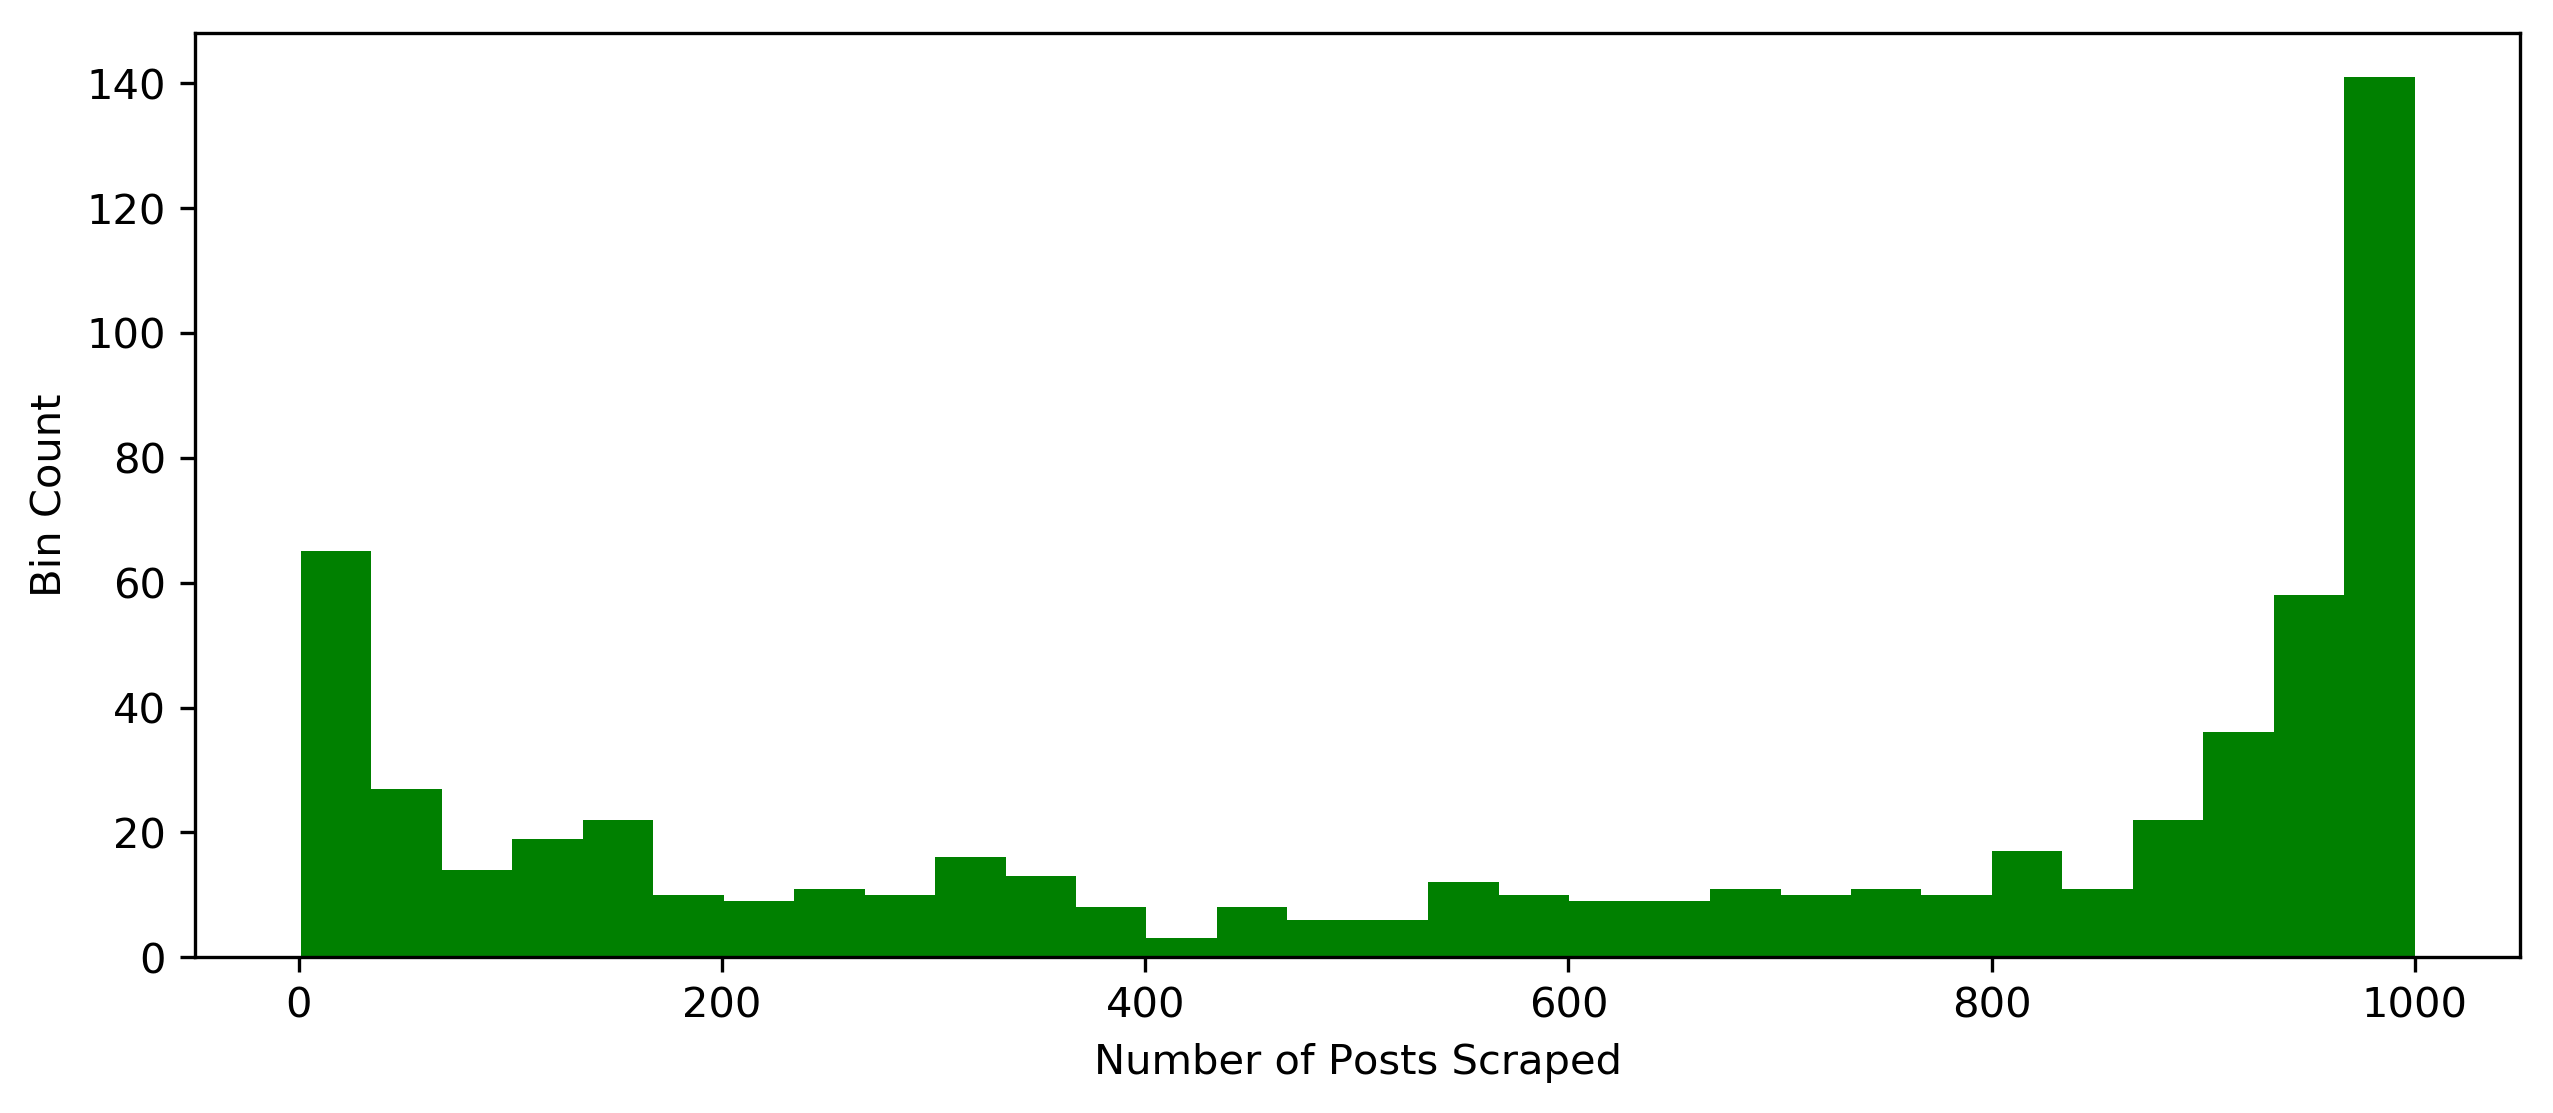
\includegraphics[width=\columnwidth]{images/Posts_Per_Page_Histogram.png}
    \caption{Histogram of the Number of Posts Scraped Per Facebook Page}
    \label{fig:histogram_posts_scraped}
\end{figure}

After obtaining advertiser pages on Facebook, this research scraped user engagement data from each Facebook page. This research uses a Python web scraper to crawl the Facebook brand pages. Facebook provides the Graph API, a publicly-available API, for accessing Facebook data. The crawler scrapes the most recent one-thousand posts from each brand page. While some pages contain more than one-thousand posts, we felt that one-thousand posts per advertiser is sufficient data per brand page. The histogram for the number of posts scraped per brand page are shown in Figure \ref{fig:histogram_posts_scraped}. In total, the study collected 366,415 Facebook posts and 1,305,375 million comments. This study collects a great deal of brand-page data via more than 350k Facebook posts and 1.3 million comments.

\subsection{Data Quality}

The study ensures data quality by relying on existing, third-party resources who specialize in both sourcing and providing data. For example, Hootsuite is a company that specializes with advertising on social media across multiple platforms. By collecting brand page URLs from Hootsuite, the study ensures its data comes from advertising pages. Another example of sourcing data is the use of Facebook's API to collect post data. Given a public Facebook page, the Facebook Graph API allows apps to pull Facebook data. The extracted data is performed by the platform itself, ensuring accuracy, and is provided in an easy-to-digest manner, aiding with data processing. The study utilizes existing businesses and resources for compiling this study's data.

The study performed manual checks to verify the correctness of both Facebook brand pages and their post statistics. The study reviewed many Facebook brand pages to ensure the pages are brand pages. On Facebook, many brand pages have alternative URLs, where instead of using their brand page id, Facebook allows them to use the name of their brand for the URL. For string URLs, the study checked to ensure that a reasonable number of those strings represent a business on Google via making requests with Python. For example, Nike's Facebook page is at https://www.facebook.com/nike, and the study can verify that nike.com is indeed a valid website. The study includes both manual and automatic checks to ensure its analysis is representative of Facebook brand pages.

When analyzing provided text data, the study uses a third-party tool, which specializes with social media text data, for generating text sentiments. This study uses the Python library VADER to perform text sentiment analysis. Text sentiment rates the orientation of the text as either negative or positive and machine learning tools are commonly used for generating text sentiments \cite{HADDI201326}.  VADER is a a parsimonious, rule-based model for Sentiment Analysis for social media text data \cite{Gilbert}. VADER's output is a score between -1 and 1 to denote the text's positive or negativity, where 1 denotes a positive sentiment, 0 is neutral, and -1 denotes a negative sentiment. The machine learning models predict the average user sentiment for the Facebook post. The post's user sentiment is the average sentiment of all user comments, as scored by VADER. This output serves as the target value for the machine learning models. Models predict the average comment sentiment for each Facebook post. The study uses an existing text-sentiment library, which is made for social media text, to measure text sentiment.

For modeling, the study uses standard deep-learning architectures to train its NN and CNNs. These architectures are freely available to import and train via Keras, a Python machine learning library. The CNN model uses VGG16 (https://keras.io/api/applications/) and the NN is a generic Keras, deep NN with seven hidden layers. The The use of existing performant NN and CNN architectures gives us confidence the deep learning models will satisfactorily learn the data. Moreover, future research can also train with these models for extending this research.

\subsection{Data Processing}

This study follows standard text processing steps \cite{Camacho-Collados2019}, including text cleaning, creating tokens, using a port stemmer, part-of-speech (POS) tagging, lemmatization, and transforming text sentences into a td-IDF vectorizer. First, the program splits data into word tokens using whitespace as a delimiter. Next, the program grouped these tokens into sentences, lowercases words, and removes common English stopwords, as well as words with three or fewer characters. The remaining words are fed into a port stemmer, which creates word stems. These stems serve as input into a POS tagger, which provides details like noun and verb declensions. Such word details are useful in determining the sentences structure and contents. The program then extracted stems with a word lemmatizer, which takes the stem and the POS tag as input. Finally, the program fed the lemmatized text sentences to a td-IDF vectorizer. The vectorizer creates word vectors, which serve as input for the neural networks. The study takes many steps to process text data to ensure the data is informative and easily digestable for the neural network.

In a similar fashion, the study takes many steps to prepare images. Given that images are inherently highly dimensional, the study takes multiple steps to reduce each image's dimensionality. First, we used principal component analysis and reduce the number of image dimensions to 20. This preserves the image directions that contain the most data. Afterwards, the image is further precessed via denoising, which reduces noise and data size. In order to emphasize edges, the study then applies Gaussian blurring, with a standard deviation of five to each image, which both applies image blurring and emphasizes edges. Dilation and erosion are also applied to the image to remove noise in the edge space. The final result are highly filtered images that emphasize shape and edges, an example of such an image is displayed in figure \cite{processed_image}. 

\begin{figure}
\centering
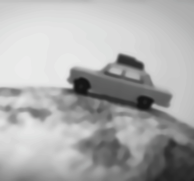
\includegraphics[width=\columnwidth]{images/preprocessed_image.png}
\caption{Example Image after Preprocessing}
\label{processed_image}
\end{figure}

This study analyzes text sentiment for posts and their comments. The post text denotes the text associated with the brand's FGC post. The comment text includes all comments made on the FGC post. Each text is scored from -1 to 1 for its positivity where -1 is negative, 0 is neural, and 1 is a very positive sentiment. The comment sentiment is averaged for each post and represents the user sentiment toward the post. Figure-\ref{comment_sentiment_histogram} shows a histogram of comment sentiments for the Facebook posts. The study rates the sentiment of user response toward a Facebook post as the average sentiment of its comments.

The sentiment dataset consists of 201,215 posts. These posts contain comment count, share count, and comment sentiment data. Of those posts, the study collected and trained on 1,305,375 million user comments. The study collected many Facebook brand posts and many more user comments.

\subsection{Brand Page Variable Correlations}

The study considers brand page variables and how it might affect user engagement. Specifically, the study explores whether general brand page characteristics are correlated with user engagement. For example, do more popular brand pages also receive more engagement. The study documents these correlations and notes how they might affect the results.  

Two brand page variables had correlations with user engagement: fan count and the number of users talking about a brand page. Unsurprisingly, these two variables are highly correlated with one another with a 0.38 adjusted r-squared. Concerning user engagement, the variable most correlated with user engagement is 'talking about count.' When users talk about a particular brand, they are more likely to share (0.22) its posts. The highest correlation is between comment count and comment sentiment, which means that posts which elicit positive user comments also receive a greater number of comments. The study found multiple correlations between Facebook page statistics and user engagement.

% here

\subsection{Modeling}

There are three types of models, text, image, and combined models. The text model uses a neural network architecture with seven hidden layers and the CNN uses the VGG16 architecture. There are two types of combined models, a decision-tree based model and an ensemble of the NN and CNN models. There are three training datasets for share count, comment, count, and comment sentiment. Training each of the four architectures on the three data types makes for a total of twelve models. This study trains four model architectures, based on different data types.

Given the study's data contains continuous variables, such as the count of shares, comments, and range of comment sentiment from -1 to 1, the study uses regression to optimize the ml models. The study uses Mean Squared Error (MSE) as its loss function for the machine learning models, which heavily penalizes values straying from the observation. The result are models with a smaller prediction range but which is able to predict which posts will outperform others. The study trains regression ml models that learn to predict if a post will perform well on social media.

The study chose hyperparameters for its models to achieve quicker training and reasonable results. Each model is iteratively trained with large batch sizes of 256 until the test dataset stops learning or its performance decreases. This research initially experimented with word vector sizes from 1k-400k. Good performance and fast training occurred with a word vector size of 10k. The NN models used 10k as the word vector size. CNNs took weeks to train with a GPU, with the NN models training in a few days. The ensemble combined model concatenates both text-based NN and image-based CNN. Each model, its use, and methods for training and testing are publicly available on Github at https://github.com/cpluspluscrowe/Masters\_Thesis. The study makes use of common or default hyperparameters for training the readily available and imported architectures.

\section{Results}

The results display the MSE for the twelve ml-models. The twelve models use a combination of different data types as input, including only-text, only-video, and a combination of text and video data. The relative MSE for the twelve models is shown in Table \ref{mse_ratios}. The combined models include a decision tree and an ensemble CNN and NN. The study provides relative MSE performance across both different architectures and combinations of input data types. Rather than provided raw MSE across all models, we provide ratios.  We also provide a histogram of the MSE to provide an understanding of how well the model performs on the test datasets.

\begin{table}[]
\centering
\begin{tabular}{lllll}
Metrics / Model & Text-Based NN & Image-Based CNN & Combined Decision Tree & Combined NN \\
Share Count       & 3.44 & 1.01 & 2.58 & 1.00 \\
Comment Count     & 1.02 & 1.01 & 1.29 & 1.00 \\
Comment Sentiment & 1.42 & 1.14 & 4.20 & 1.00
\end{tabular}
\caption{\label{mse_ratios}Model Mean Squared Error Reported as a Ratio to the Best Model's Performance}
\end{table}

The combined model best predicted all user behavior metrics. Each machine learning model had its lowest MSE predicting for share count. The CNNs achieved a lower MSE than the NN on all metrics. Moreover, the CNN performance is best on data exhibiting a higher variance. Figure \ref{share_count_histogram} and \ref{comment_sentiment_histogram} show the predicted vs actual distribution for the combined model.

The decision tree performed far worse than the combined model. While the exact reason is unknown, there are a few differences between the two models. First, the combined model closely integrates with the text-based NN and image-based CNN. Second, when the combined model trains, it also trains its two-parent models. As a result, the decision tree did not learn alongside its inputs. Likely, parent models compensate for mistakes by training together.

\subsection{Discussion}

\subsubsection{RQ 1: Ability to Predict User Engagement}

Popular pages do not generate more comments per post. This might capture a phenomenon where brands receive many followers but produce less interesting content. Therefore generating many followers does not necessitate an engaged user base. The opposite effect is also seen where brands have entire social media teams that produce high quality content that in turn generates a lot of engagement. On social media, a large page also needs to produce quality content in order to generate user engagement.

Correlations exist in the occurrence of some user engagement metrics. Principally, there is a general correlation between user comment sentiment and other metrics, specifically comment count and share count. However, the correlation between comment and share count is much weaker. The implication is that posts that elicit positive comments will also receive a greater number comments and shares. 

\begin{figure}
\centering
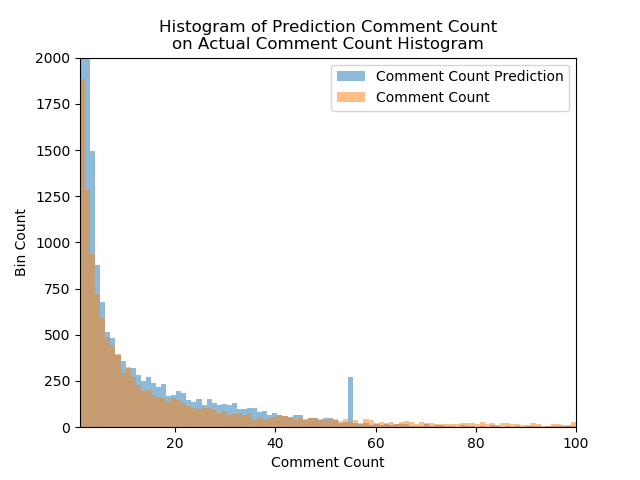
\includegraphics[width=\columnwidth]{images/Comment_Count_Prediction_vs_Actual.png}
\caption{Actual vs Predicted Comment Count Histogram}
\label{comment_count_histogram}
\end{figure}

\begin{figure}
\centering
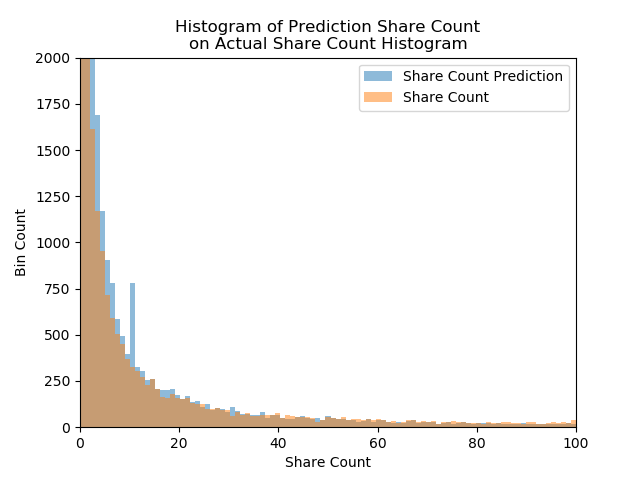
\includegraphics[width=\columnwidth]{images/Share_Count_Prediction_vs_Actual.png}
\caption{Actual vs Predicted Share Count Histogram}
\label{share_count_histogram}
\end{figure}

\begin{figure}
\centering
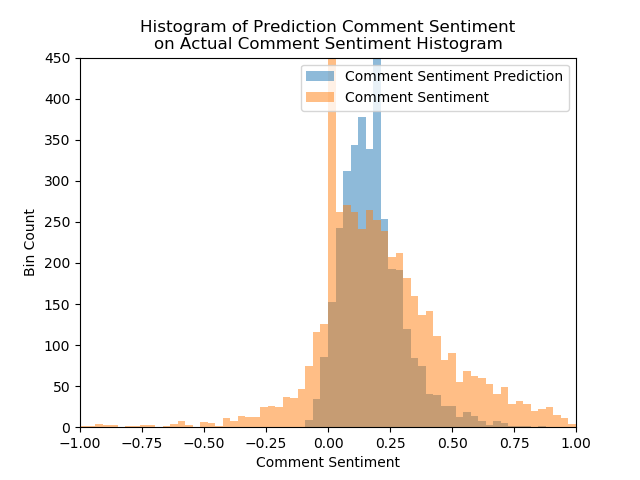
\includegraphics[width=\columnwidth]{images/Sentiment_Prediction_vs_Actual.png}
\caption{Actual vs Predicted Comment Sentiment Histogram}
\label{comment_sentiment_histogram}
\end{figure}

The models perform the best on distributions that skew toward fewer counts, such as comment and share counts. These are distributions that resemble the geometric distribution; those that heavily decrease for higher counts. The actual vs predicted histograms look very similar and how lower model losses, as shown in Figure \ref{share_count_histogram} and Figure \ref{comment_count_histogram}. Models do especially well at predicting share count and comment count on Facebook brand posts.

The model achieves a quite low model loss for predicting user sentiment for posts. This is largely possible due to the close relationship between post sentiment and comment sentiment. The resulting actual vs predicted comment sentiment is shown in Figure \ref{comment_sentiment_histogram}. The study successfully predicts comment sentiment for Facebook brand posts.

\subsubsection{RQ 2: Performance of Images vs Text}

Image-based models outperform text-based models the most when predicting share count. The share count metric resembles a geometric distribution where most posts have very few shares, similar to comment count. However, share count has a higher variance than comment count. The inference is that image-based models did better at handling the variance within the metric share count. It is noting that even a simple decision tree with image data outperforms a deep neural network with text data for predicting share count. Image data seems especially useful for producing shares, which is reflected in the better performance of image-based models. Image-based models show a greater ability at handing distributions with more variance.

Both text-based NN and image-based CNN perform almost equally well for predicting comment counts, i.e., they achieve a similar MSE. Both models receive the same input in terms of word vectors and both models are able to process this data. The similar performance might mean that both models similarly process the data or tend to find the same patterns in the existing data. Both text-based and image-based models perform similarly for predicting comment counts.

The combined decision tree performed poorly compared to all other models on almost all metrics. The combined decision tree's poor performance indicates the complexity of the input data, both word and image vectors. A decision tree is likely a poor candidate for handling more complex inputs, however, one might expect it would be able to find patterns in comment sentiment, which has more simple inputs based on parts of speech. Nevertheless, the decision tree even performed poorly when predicting comment sentiment. The combined decision tree is unable to learn the patterns within the provided word and image vectors for predicting user engagements.

Image-based models performed better than text-based models on all metrics, likely because it emphasizes images' importance for predicting user interaction on social media. Text-based models were poor predictors for many metrics. Text-based models did especially badly in prediction share counts. One may guess that users are sharing content they consider worthy of sharing.

One consideration might be that both NN and CNN show a similar performance on the data but major improvements can be made in terms of share count and comment sentiment in the use of a model that combined both image and text data. The 14\% improvement for comment sentiment and 3.5x improvement on share count can be made across either the NN or CNN. The combined model demonstrates dramatic  improvement on at least one metric for each of the single-data type models.

\subsubsection{RQ 3: Ability to Distinguish Between Higher and Lower Performing Ads}
In light of the newly created data, there are no other baseline measures for what constitutes good model performance. One goal was to produce a model that performed better than random guessing. Random guessing alone is not representative of the data. A better guess is based on the input's distribution. A good random guess would consider the data's value at each point along with its distribution. Such a distribution would weigh each value by the frequency of data. This calculation is the expected value. For a normal distribution, the expected value is equal to the mean. Also, each output in the research resembles the normal distribution after a log transformation. If the model always predicts the mean, the MSE is equal to the data's variance. The variance is a squared order of the data's distance from the mean. The MSE is also a squared order of the model's prediction from the actual value. Producing a model whose loss is below the variance is a general measure of demonstrating the model is doing a significant amount of learning. Fortunately, the combined model's performance was always much lower than each output data's variance.

Models with a higher variance achieved the worst overall loss/variance ratio.  It seems that the larger the data variance, the higher the resulting mode's MSE.  Share count had the highest variance of all the measured metrics, 1000x more than the comment count.  The high MSE likely reflects that share counts are less related to the image and text data. Share counts might be a factor of other features, like page popularity.

\subsubsection{Use Case}
The research applied the models in a real-world application. The application explored a use case to demonstrate the model's ability to choose which two advertisements will receive the greatest user engagement. The research found that models are unlikely able to differentiate between advertisements with similar performances. However, this research is able to consistently differentiate between ads with larger difference. This research shows that the model can differentiate a difference in ad performance for ads with at least a standard deviation difference in user engagement. The combined model performs all predictions since it performed best across all metrics. Moreover, the application is the most useful if it can detect poor-performing and best-performing advertisements.

The scenario is predicting user engagement for advertisements. The scenario pairs Facebook posts together. The model predicts user engagement for all posts. The program scores how often the model correctly predicted for greater user engagement. The program reports the result for each metric. The score is the number of correct predictions over incorrect predictions. This research compared the score with a random model, which would produce the correct answer 50\% of the time. The combined model scored 93\% for comment sentiment, 65\% for comment count, and 63\% for share count. The prediction model is able to consistently predict which of two advertisements will receive the most positive user comments.

The model performance shows its applicability in the real world.  Platforms could employ the models to aid advertisers in choosing the best performing advertisement before paying to advertise it on social media. The model can tell advertisers which ads would perform best on the platform, which allows advertisers have their ads vetted. The vetting could prevent advertisers from spending large amounts of money showing worse ads. Moreover, the vetting would allow advertisers to only show ads that will perform best. In the context of billions, 93\%, 65\%, and 63\% accuracy is a substantial monetary difference.

\subsection{Study Contributions}

The research found that machine learning with both image and text data results in enormous improvements for predicting comment sentiment. The combined model showed a 14\% increase in predicting user combined sentiment vs. the text-based NN and image-based CNN. The implication is that a combination of image and text data is best when predicting how users will respond to an advertisement. The study found significant gains in the performance of a model combining image and text data when predicting user sentiment.

The study found that text-based models can be improved by 42\% for comment sentiment and a factor of 3.5x for share count. Both the image and combined models far outperformed text-only models for comment sentiment and share count. Text models that ignore image post data are likely missing large opportunities for improved model performance from incorporating image data via a CNN. 

The study demonstrates an accuracy of 93\%, 65\%, and 63\% for comment sentiment, comment count, and share count when predicting which of two advertisements will receive a greater amount of user engagement. This provides an application of the research on the combined model for advertisements. Advertisers can expect tangible gains in predicting user engagement when utilizing ml models that predict user engagements based on post text and image data. 

Given that many studies only use one data types: either images or text, this study provides both an insight and a methodology for how one might go about improving their model's performance. The study the use of an ensemble model of NN and CNN achieved an improved performance across all metrics. The study also provides its architectures, hyperparameters, and code examples for the models. This study demonstrates the degree of improvement that a combined model can achieve for predicting user engagement on advertisements.

\subsection{Limitations and Future Work}
% existing models were not publicly available.

The study is not able to acquire existing ml models and study data concerning single-data type models. The data and models are not for public use. The result is that this study made use of existing, high-performing model architectures for both CNN and NN. This allows the study to ensure its results are repeatable. Using pre-existing model architectures also ensures that existing research's best practices for ml models and architectures are included within this study. The study is not able to show the improved benefit of the combined model on pre-existing study data or models, however, the study makes use of well-known architectures to ensure model performance and study replicability. 

Given that share count and comment-sentiment have a coefficient of determination over 0.4, the share count model is likely a good input for predicting comment sentiment. Future research can incorporate this input to improve future models when predicting user behavior. In addition, future research could overcome existing Facebook API scraping problems. Another avenue for research is collecting comment sentiments for the 350k Facebook posts and using the new data to train better models.  Moreover, future work can incorporate the combined text and image model with the image-based CNN and text-based NN into an ensemble model to see if it improves performance.

The models created from this research could generate data to train a generative model.  The generative model could transform images and text into advertisements that should generate more user interaction.  The transformed and original advertisements could both be shown on social media and their user interactions compared. Thus, the study might demonstrate that generative models generate and improve existing advertising content.

\bibliographystyle{informs2014}
\bibliography{references.bib}

% Acknowledgments here
%\ACKNOWLEDGMENT{%
% Enter the text of acknowledgments here
%}% Leave this (end of acknowledgment)


% Appendix here
% Options are (1) APPENDIX (with or without general title) or 
%             (2) APPENDICES (if it has more than one unrelated sections)
% Outcomment the appropriate case if necessary
%
% \begin{APPENDIX}{<Title of the Appendix>}
% \end{APPENDIX}
%
%   or 
%
% \begin{APPENDICES}
% \section{<Title of Section A>}
% \section{<Title of Section B>}
% etc
% \end{APPENDICES}

% References here (outcomment the appropriate case) 

% CASE 1: BiBTeX used to constantly update the references 
%   (while the paper is being written).
%\bibliographystyle{informs2014} % outcomment this and next line in Case 1
%\bibliography{<your bib file(s)>} % if more than one, comma separated

% CASE 2: BiBTeX used to generate mypaper.bbl (to be further fine tuned)
%\input{mypaper.bbl} % outcomment this line in Case 2

\end{document}


